\chapter{Legolas applications} \label{ch: legolas_applications}


\graphicspath{{05-applying_legolas/figures/}}

\begin{chapterquote}[Robert C. Martin][Clean Code: A Handbook of Agile Software Craftsmanship][]
  Why do most developers fear to make continuous changes to their code? Because they are afraid they'll break it.
  Why are they afraid they'll break it? Because they don't have tests.
\end{chapterquote}

\usespublishedwork{
  Most of this Chapter was published in ``Legolas: a novel tool for magnetohydrodynamic spectroscopy'', 2020, \apjs,
  251, 25 \citep{claes2020_legolas}. N. Claes developed {\legolas} in close collaboration with J. De Jonghe, generated the data and figures and wrote a first draft of the manuscript; J. De Jonghe revised and extended the manuscript. R. Keppens contributed to the revision of the paper.
}

In the previous Chapter we discussed the mathematical formalism behind {\legolas}. As is common practice when developing a brand new numerical code we now have to test the implementation against various known results. This Chapter will mostly be dedicated to the validation of our new numerical tool, by comparing numerical spectra with known results from theory and/or the literature. Additionally, we will briefly touch upon the extensive (and continuous) testing framework {\legolas} uses.

\section{Introduction}
Any piece of software, both existing and newly developed, should be accompanied by a decent testing framework to ensure that any changes made to the code, either in the present or in the future, do not break things that were previously working fine. It is easy to develop a piece of code, it is less easy to develop a \emph{working} piece of code, and finally it is certainly not enough for code to just ``work''. Every part of the implementation should be tested against known results in order to make sure that the code actually does what it is expected to do. In an ideal world, every single line of a code base is tested at least once, while at the same time also accounting for various branches in the logic.

In this Chapter we validate {\legolas} against a plethora of test cases, thereby ensuring a correct treatment of the governing equations. Depending on which physical effects are taken into account, we know a priori some general spectral properties that should hold, and we can thus test the properties of the obtained spectra against our predictions. For eigenmode quantifications of ideal, static MHD configurations under adiabatic conditions, we know that the static -- that is, no equilibrium flow -- and adiabatic linear MHD equations make the problem self-adjoint. When performing a standard Fourier analysis in the ignorable directions, the resulting eigenvalue problem is then Hermitian, meaning that all eigenfrequencies will be either fully real (stable waves) or fully complex (pure damped or unstable modes), hence they are found on the real or imaginary axis of the complex eigenfrequency plane, and the full MHD spectrum will be both left-right and up-down symmetric. The inclusion of nonideal effects like resistivity or thermal conduction lifts the self-adjointness of the eigenvalue problem, allowing the eigenmodes to move away from the axes into the complex plane, and the up-down symmetry gets broken. As long as the equilibrium configuration is static, all (adiabatic or non-adiabatic) modes will still have a complementary mode that lies mirrored around the imaginary axis, making the entire spectrum left-right symmetric. This is related to the forward and backward propagating mode symmetry, or the equivalent statement on the parity-time (\gls{PI}) symmetry.

The inclusion of a background flow breaks the left-right symmetry of the MHD spectrum, resulting in an even more complicated spectral structure. However, the study of the ideal, linear MHD spectrum is flowing plasmas is still governed by a pair of self-adjoint operators \citep{goedbloed2011,book_MHD}, and it leaves the up-down symmetry of the spectrum intact (where every overstable mode has an equivalent damped counterpart at the same frequency).

The actual validation of the code should follow a stepwise approach, where we first test the most simple cases. This is dictated by common logic: if even the most simple cases do not work, then we can never expect correct spectra for more complicated equilibria. Hence to begin with, we discuss results for adiabatic equilibria where only gravity is included. In this case we can compare numerical spectra obtained through {\legolas} with analytical solutions acquired by solving dispersion relations; here, we first focus on stratified atmospheres containing $p$ and $g$ modes. We then move on to cylindrical geometries, where we first look at adiabatic flux tubes, followed by the inclusion of flow effects by considering equilibria known to be susceptible to KHI and Suydam cluster modes. Next, our focus shifts to nonadiabatic effects by looking at a resistive MHD calculation for a case without gravity, where the value of a quasi-mode is known analytically. Resistive tearing modes are also discussed, combining the effects of flow and resistivity. Finally we will treat the inclusion of thermal conduction and optically thin radiative cooling effects, where we look at nonadiabatic discrete Alfv\'en waves and magnetothermal modes.


\section{Cartesian cases: waves in stratified atmospheres}
First of all we discuss multiple theoretical results for adiabatic equilibria in a Cartesian geometry, where only gravity is included. We consider $p$ and $g$ odes in stratified layers and pay special attention to specific unstable branches.

\subsection{Gravito-MHD waves} \label{ss: gravito-mhd}
The first test case covers gravito-MHD waves as discussed in \citet[Figure 7.9]{book_MHD}, which handles an exponentially stratified atmosphere with constant sound and Alfv\'en speeds. This magnetised atmosphere contains the generalisation of the $p$ and $g$ modes of an unmagnetised layer, and the constancy of the sound and Alfv\'en speed renders this particular configuration analytically tractable (even though it has an inhomogeneous density profile), because the slow and Alfv\'en continua collapse to points. the geometry is Cartesian with $x \in [0, 1]$ and an equilibrium configuration given by
\begin{equation} \label{eq: gravito_mhd}
  \begin{gathered}
    \rho_0 = \rho_c \exp\left(-\alpha x\right), \qquad p_0 = p_c \exp\left(-\alpha x\right), \\
    \bb_0 = B_c \exp\left(-\frac{1}{2}\alpha x\right)\unit{z}, \qquad \alpha = \frac{\rho_c g}{p_c + \frac{1}{2}B_c},
  \end{gathered}
\end{equation}
where $p_c$ and $B_c$ are taken to be 0.5 and 1, respectively, as to yield a plasma beta equal to unity. The parameter $\alpha$ is taken to be 20, which, together with $g = 20$, is used to constrain the value for the constant $\rho_c$. These four equations completely determine the equilibrium configuration, because the temperature is $T_0 = p_0/\rho_0$, following the ideal gas law. The spectrum discussed in \citet{book_MHD} is actually the solution to the analytic dispersion relation for gravito-MHD waves, which shows the squared eigenvalue as a function of wavenumber for a fixed angle $\theta = \pi / 4$ between the wave vector $\bk_0$ and the magnetic field $\bb_0$. However, the spectrum as calculated by {\legolas} corresponds to one single equilibrium configuration, meaning one value for $k_y$ and $k_z$. In order to reproduce Figure 7.9 from \citet{book_MHD} and compare the results, we performed 100 different runs where the equilibrium parameters in Equation \eqref{eq: gravito_mhd} remained unchanged, but $k_y$ and $k_z$ took ok 100 different values between $0$ and $\sqrt{250}$ as to yield a wavenumber range for $k_0^2$ between 0 and 500. Because the magnetic field is purely aligned with the $z$-axis, we can write $\kpara = k_z = k_0\cos(\theta)$ and $\kperp = k_y = k_0\sin(\theta)$. All runs were performed using 351 gridpoints, yielding a matrix size of $5616 \times 5616$.

\begin{figure}[t]
  \centering
  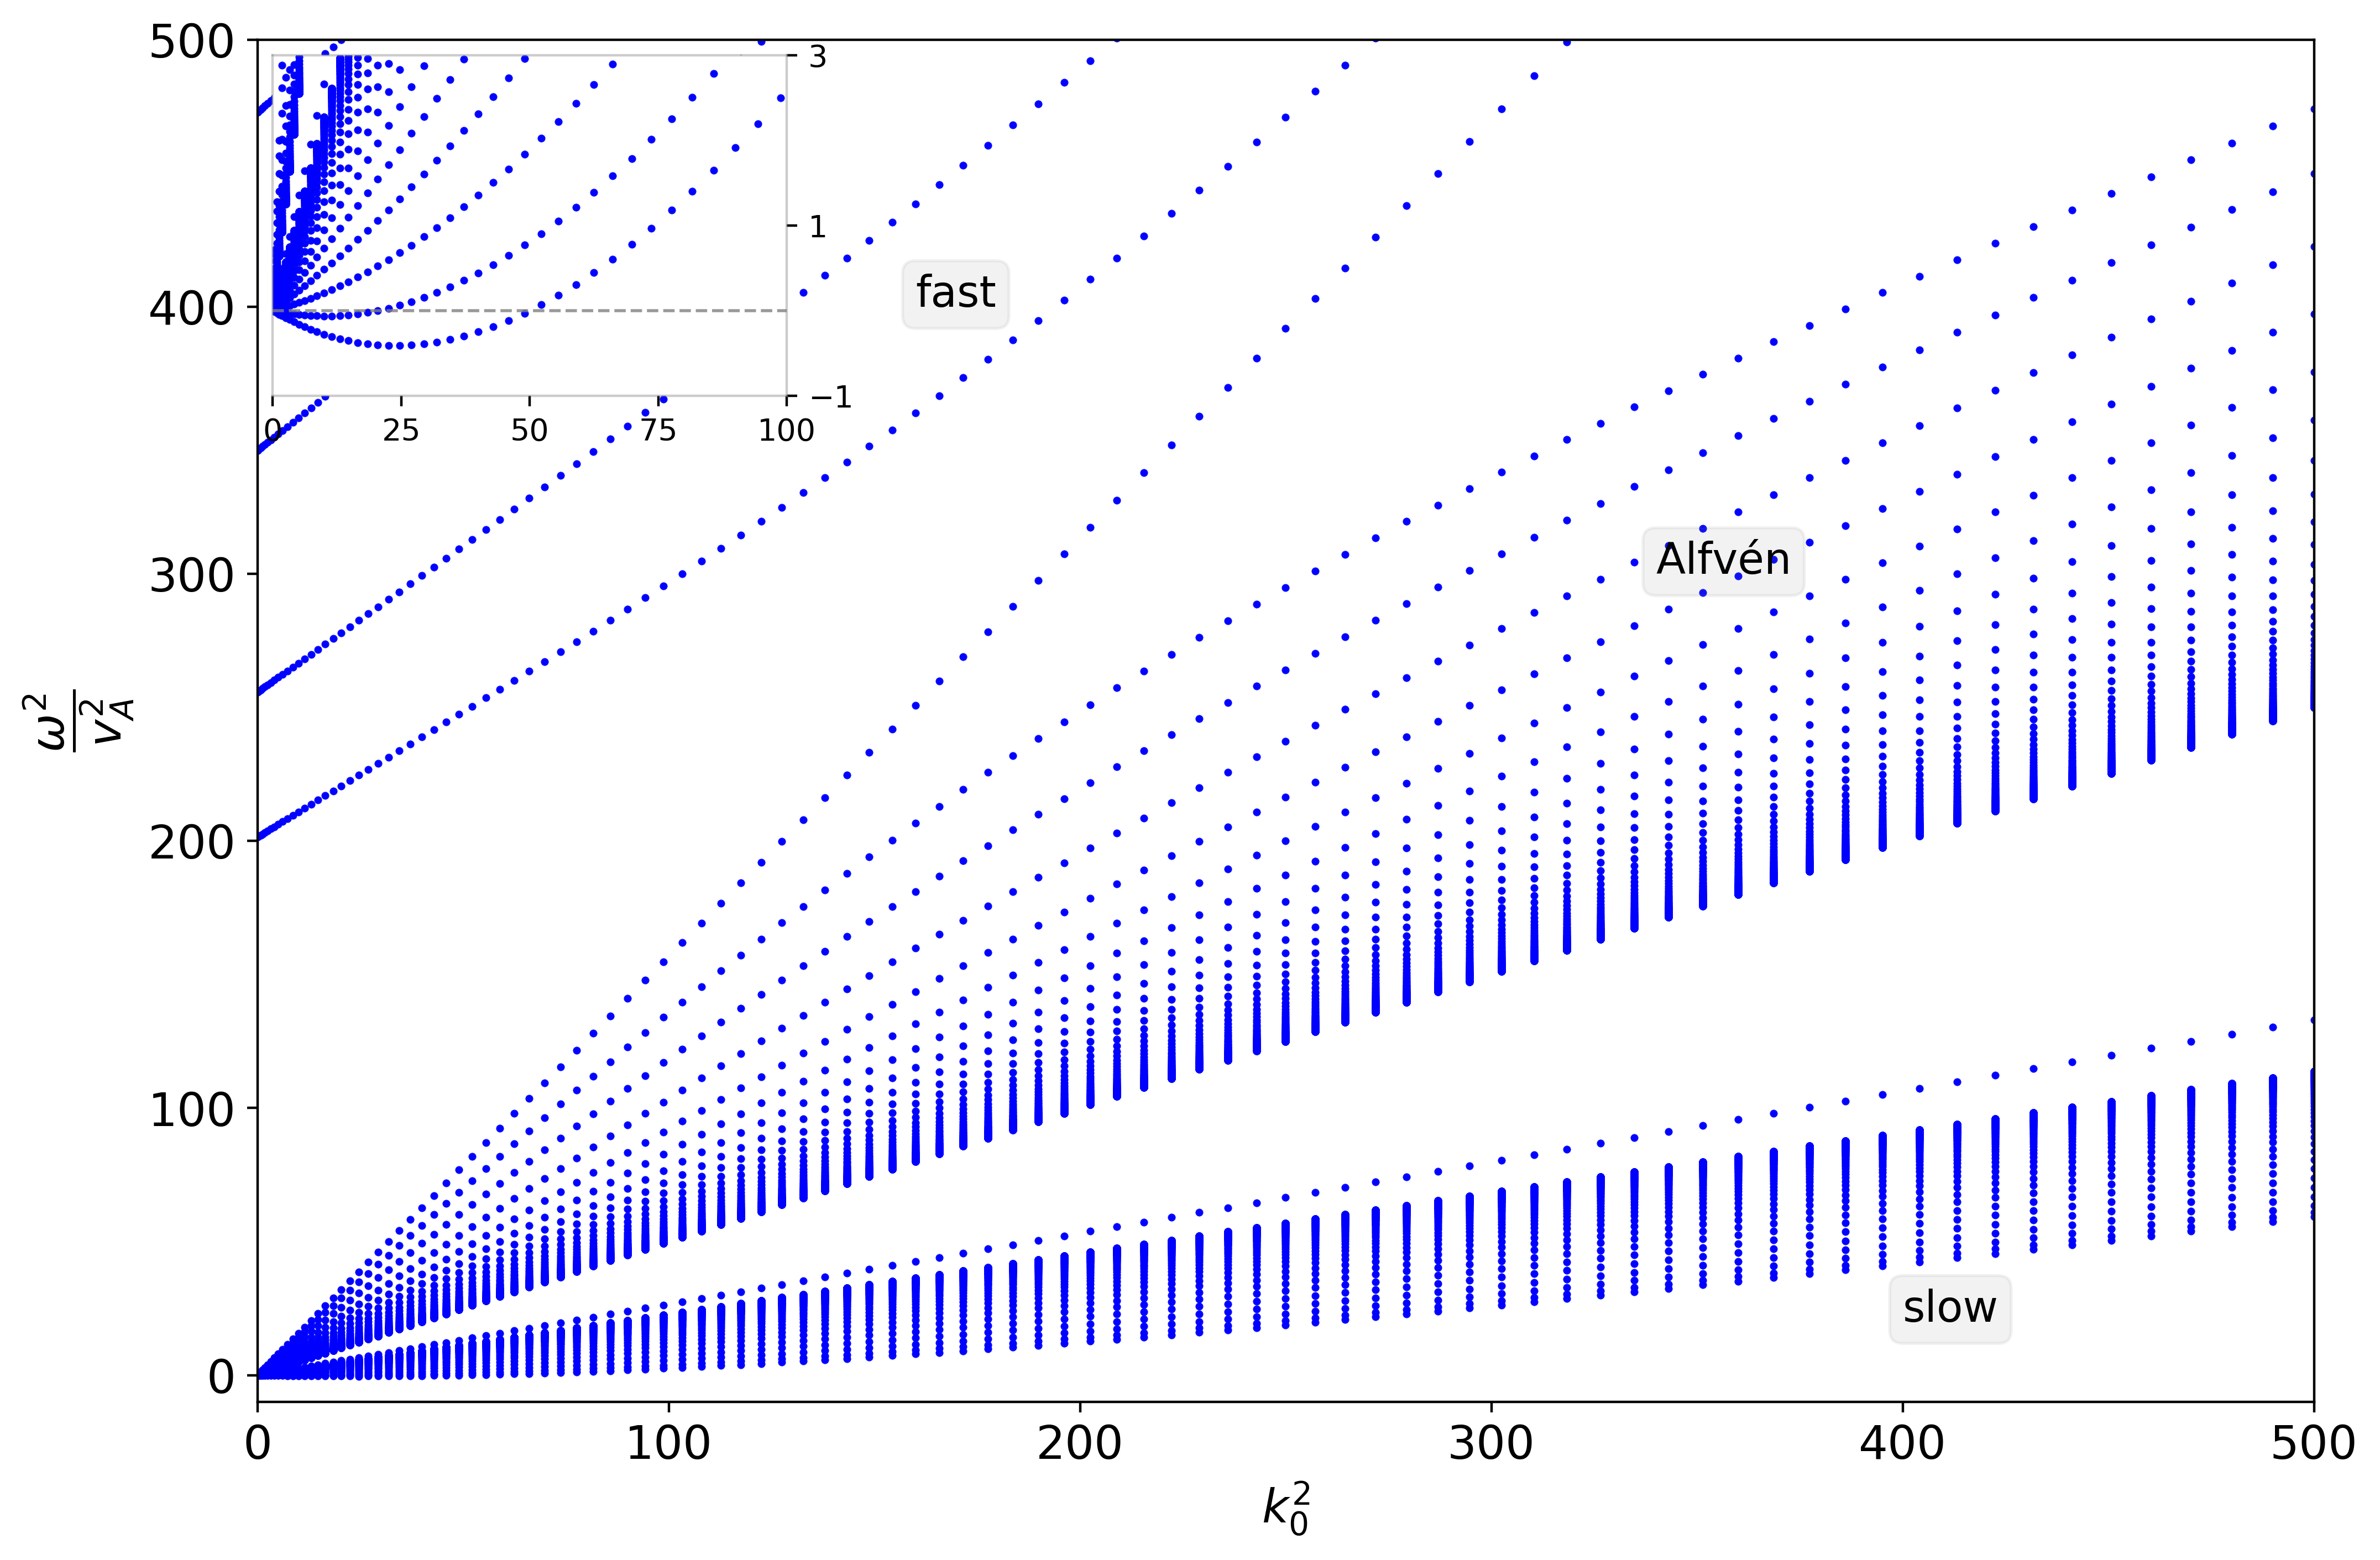
\includegraphics[width=\textwidth]{gravito_mhd.png}
  \caption{
    Spectrum of gravito-MHD modes, obtained through 100 {\legolas} runs of 351 gridpoints each. The fast (top), Alfv\'en (middle) and slow (bottom) branches of the MHD spectrum are clearly visible. The inset shows unstable slow modes at low frequencies.
  }
  \label{fig: gravito_mhd}
\end{figure}

The results are shown in Figure \ref{fig: gravito_mhd}, where every vertical collection of points at the same $k_0^2$ value represents one single {\legolas} run. Because we are in an MHD regime with a plasma $\beta = 1$, the three MHD subspectra can be clearly distinguished, showing the fast $p$ modes (top-left branches), Alfv\'en $g$ modes (middle branches), and slow $g$ modes (bottom branches). The inset shows a zoom-in near the marginal frequency of the spectrum, showing unstable $(\omega^2 < 0)$ slow MHD modes. These long-wavelength unstable modes are related to the Parker instabilities, due to magnetic buoyancy, as we will show in Section \ref{ss: quasi-parker}. Note that because this case is adiabatic and fully self-adjoint, every individual MHD spectrum is left-right and up-down symmetric in the complex eigenfrequency plane, but this aspect is hidden from the $\omega^2$ -- $k_0^2$ view shown here.


\subsection{Quasi-Parker instabilities} \label{ss: quasi-parker}
Next we discuss a modified case of the gravito-MHD waves, namely a spectrum showing quasi-Parker instabilities as done in \citet[Figure 12.2]{book_MHD}. The difference with the previous case is that a fully analytic description is no longer possible, because the introduction of magnetic shear leads to continuous ranges in the MHD spectrum. Instead of showing the spectrum for one single value for $\theta$, we now vary the direction of the wave vector $\bk_0$ between 0 and $\pi$. The equilibrium configuration is similar to the one in Section \ref{ss: gravito-mhd}, given in Cartesian geometry by
\begin{equation} \label{eq: quasi-parker}
  \begin{gathered}
    \rho_0 = \rho_c \exp\left(-\alpha x\right),
    \qquad
    p_0 = p_c \exp\left(-\alpha x\right),
    \qquad
    \alpha = \frac{\rho_c g}{p_c + \frac{1}{2}B_c}, \\
    B_{02} = B_c \exp\left(-\frac{1}{2}\right)\sin\left(\lambda x\right),
    \qquad
    B_{03} = B_c \exp\left(-\frac{1}{2}\right)\cos\left(\lambda x\right),
  \end{gathered}
\end{equation}
where magnetic shear was introduced through the parameter $\lambda$. The quantities $\alpha$ and $B_c$ are assigned the same values as in Equation \eqref{eq: gravito_mhd}; though now $g = 0.5$ and $p_c = 0.25$, which yield a plasma beta $\beta = 0.5$. The wave vectors are given by $k_y = \pi\sin(\theta)$ and $k_z = \pi\cos(\theta)$, such that $k_0^2 \approx 10$. The angle $\theta$ was varied between 0 and $\pi$ for a total of 100 runs at 351 grid points each, shown in Figure \ref{fig: quasi_parker}.

The left panels handle the case without magnetic shear, that is, $\lambda = 0$, which basically reduces to the one from the previous subsection. In this case, the slow and Alfv\'en continua collapse into single point values, denoted in red and cyan, respectively. The right panels show the same configuration where $\lambda = 0.3$ was taken, introducing magnetic shear, which introduces genuine continua seen as bands. These continua affect the overall stability and organise the entire MHD spectrum: all discrete modes are fully aware of the essential spectrum formed by these (slow and Alfv\'en) continua and the (fast) accumulation points at infinite frequency. All features of the original figure in \citet{book_MHD} are reproduced. The inset zooms into the region where both continua overlap, showing quasi-interchange and interchange instabilities. Once more, each run, shown here collectively in Figure \ref{fig: quasi_parker}, actually has a spectrum that is left-right and up-down symmetric in the eigenfrequency plane. This is depicted on Panels c and d, which show the eigenfrequency view for one single case $(\theta = 0.3\pi)$. The continuum ranges separate nicely: the collapsed single point values are denoted by cyan (Alfv\'en) and red (slow) points on Panel c, and the genuine continua are shown with cyan and red bands on Panel d. The instabilities themselves are situated on the (positive) imaginary axis, due to the self-adjointness of the eigenvalue problem.

\begin{figure}[t]
  \centering
  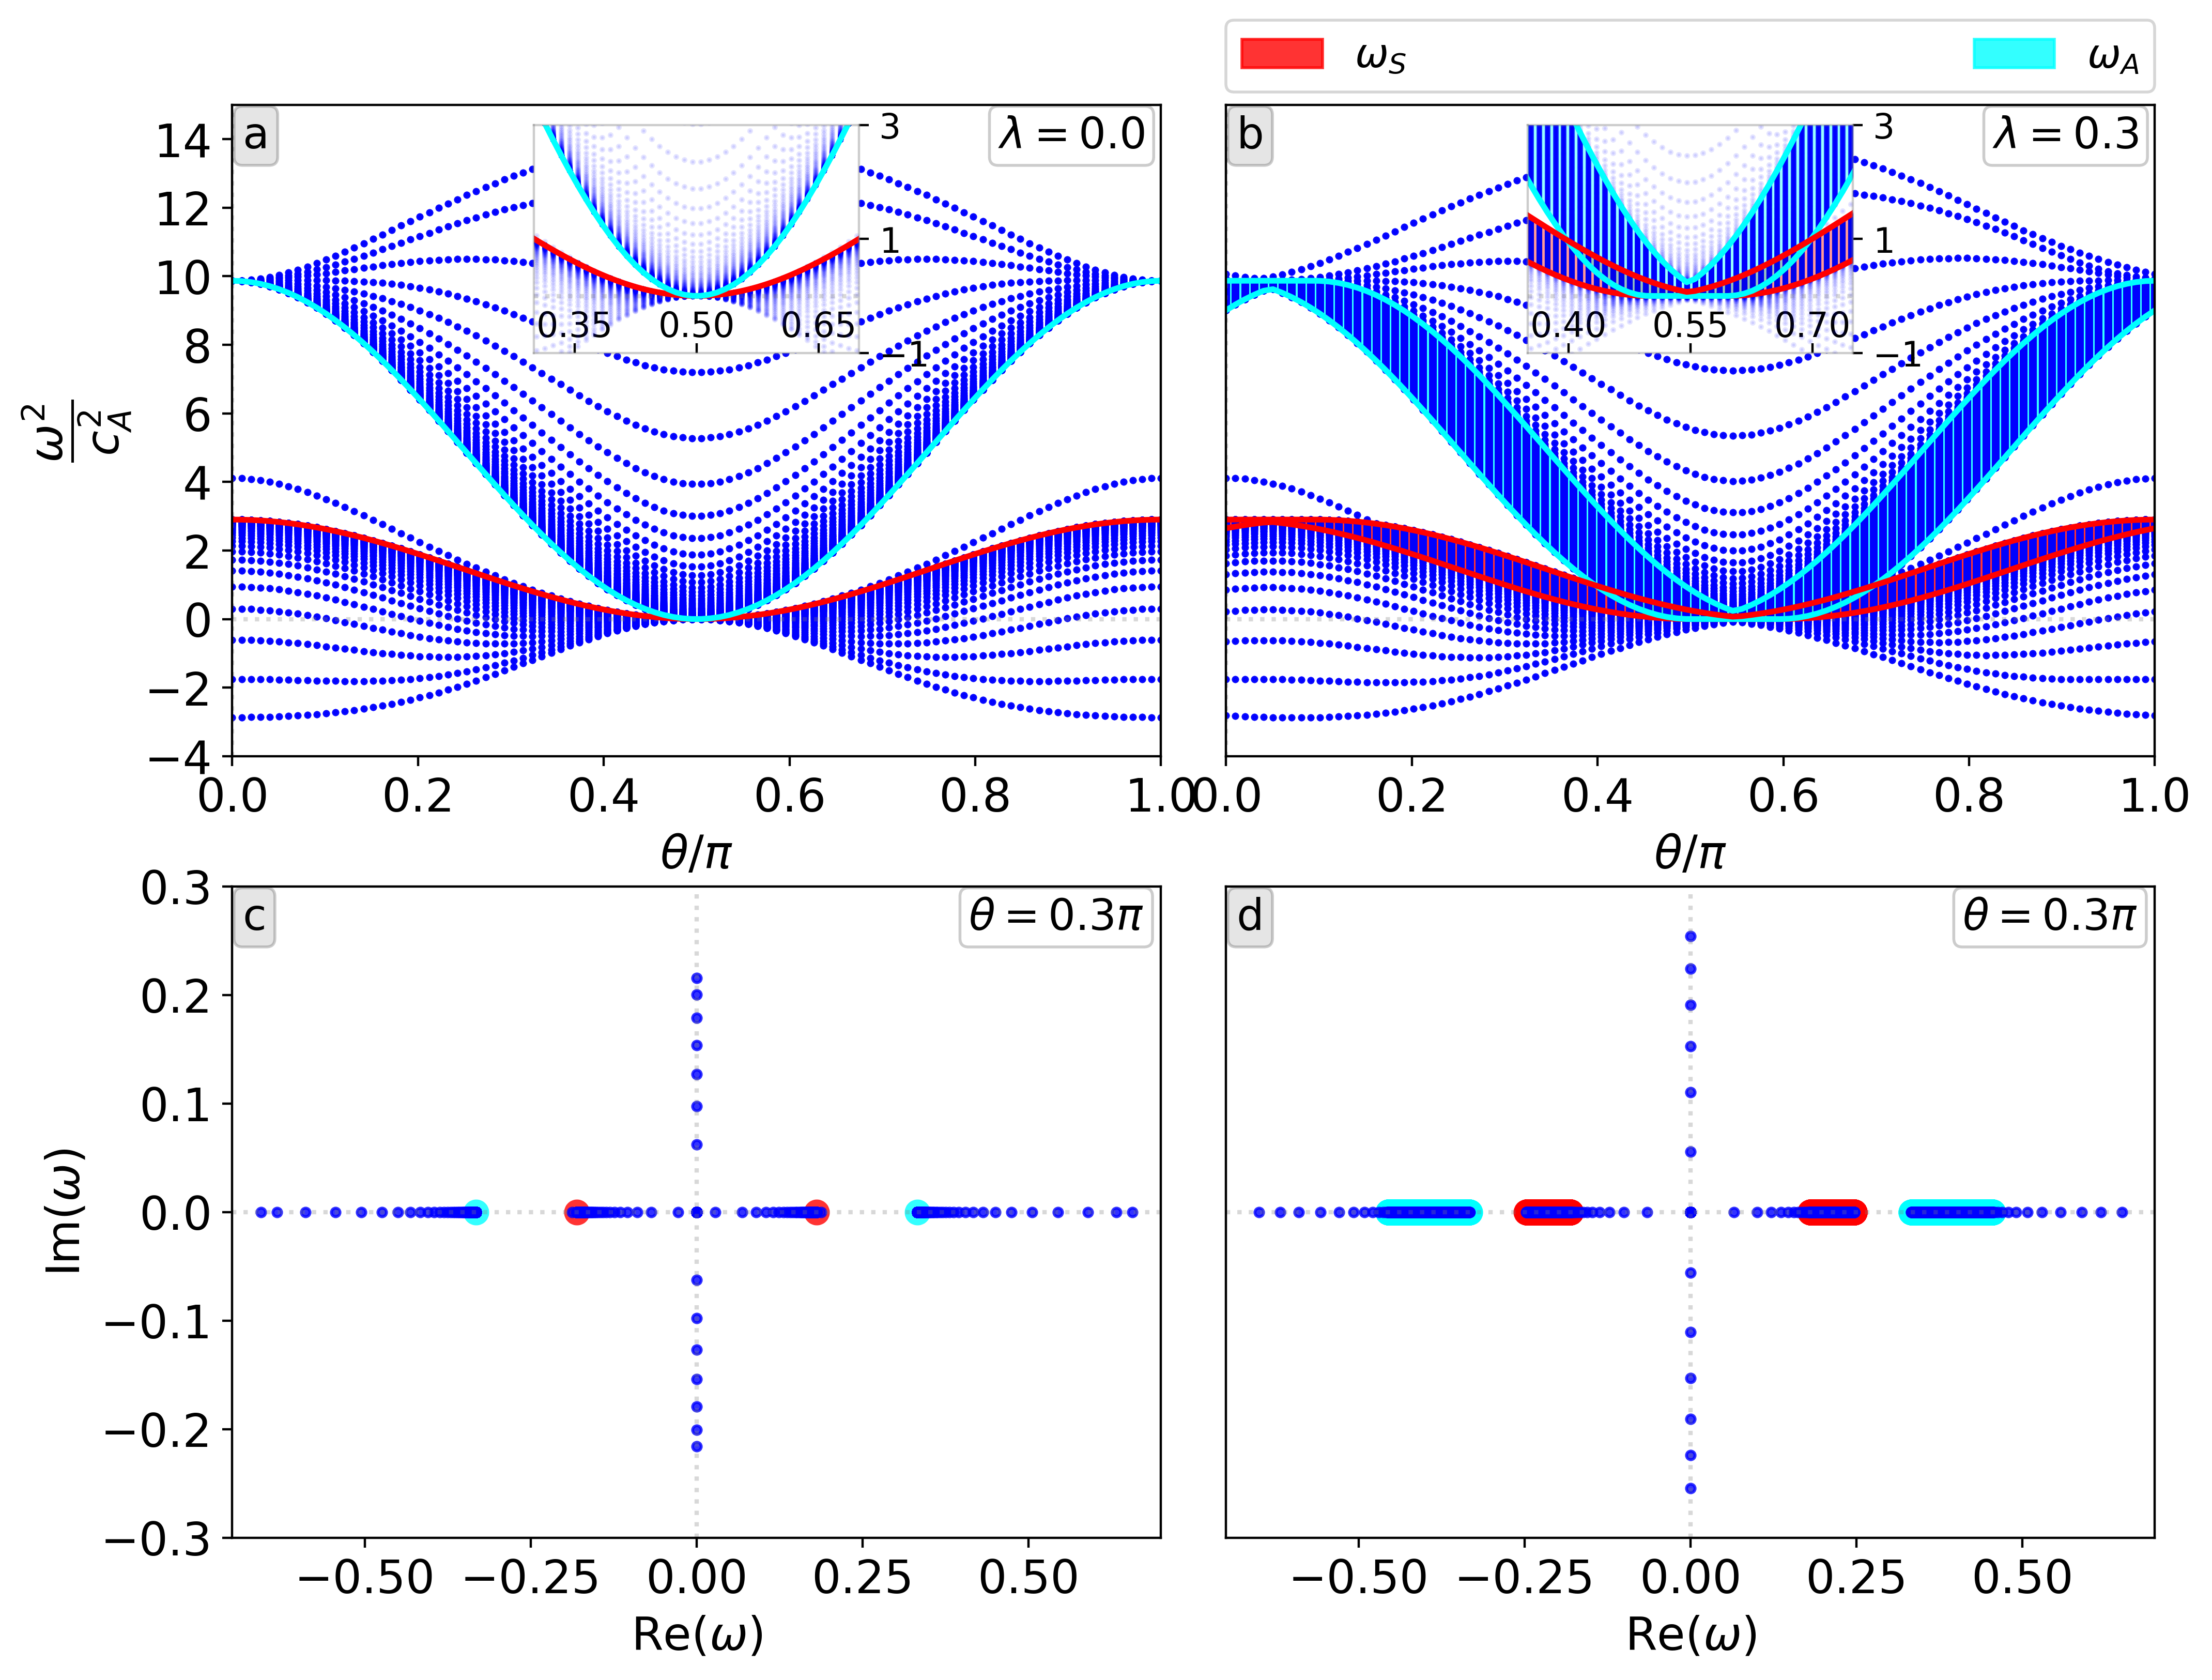
\includegraphics[width=\textwidth]{quasi_parker.png}
  \caption{
    Spectrum showing Parker and quasi-Parker modes without (\textbf{a}, \textbf{c}) and with (\textbf{b}, \textbf{d}) magnetic shear. The slow and Alfv\'en continua are shown in red and cyan, respectively, where the insets zoom into the region of quasi-interchange modes. The bottom row of panels show the eigenfrequency view for the single case $\theta = 0.3\pi$. The continua are again annotated in the panels, visualising the collapsed single point values (Panel \textbf{c}) as well as the genuine continuum ranges (Panel \textbf{d}).
  }
  \label{fig: quasi_parker}
\end{figure}

As explained in \citet{book_MHD}, we see from this eigenmode computation that the Parker instability, which is there for $\bk_0$ parallel to $\bb_0$, becomes a quasi-Parker instability away from perfect alignment and connects smoothly to well-known quasi-interchange instabilities that occur here (marginally) away from perpendicular orientation. Quantifying how the equilibrium parameters influence the growth rates of these unstable branches can only be done numerically, for example with {\legolas}.

\section{Adiabatic, cylindrical cases}
Next we move on to cylindrical configurations, which provide tests for the scale factor $\eps$ in the equations. Analytical results from the literature are again well reproduced. Furthermore, we look at different spectra previously obtained by the LEDA code, discussed in various papers, and compare those with the new spectra from {\legolas}.

\subsection{Magnetic flux tubes}
The first case that we describe in this subsection is a magnetic flux tube embedded in a uniform magnetic environment, discussed in \citet{book_roberts}. The equilibrium configuration is simple, in the sense that we have a uniform magnetic field aligned with the $z$-axis both inside and outside of the flux tube, with a similar structure for the other equilibrium parameters:
\begin{equation}
  B_0(r), \rho_0(r), p_0(r), T_0(r) =
  \begin{cases}
    B_0, \rho_0, p_0, T_0, \qquad &r < a \\
    B_\text{e}, \rho_\text{e}, p_\text{e}, T_\text{e}, \qquad &r > a
  \end{cases}
\end{equation}
where the subscripts ``0'' and ``e'' refer to values inside the tube and for the environment, respectively. The outer radius of the tube is denoted by $a$ and hence represents a discontinuous interface between the tube itself and the environment. Because total pressure balance should be preserved across the boundary, which is something that follows from Equation \eqref{eq: force_equilibrium}, this yields a relation between pressures and magnetic field components inside and outside of the tube, which in turn implies a connection between the plasma densities, sound speeds, and Alfv\'en speeds across the boundary:
\begin{equation} \label{eq: flux_tube_pbalance}
  p_0 + \frac{1}{2}B_0^2 = p_\text{e} + \frac{1}{2}B_\text{e}^2, \qquad\qquad
  \frac{\rho_e}{\rho_0} = \frac{\soundspeed^2 + \dfrac{1}{2}\gamma \alfvenspeed^2}{
    c_\text{se}^2 + \dfrac{1}{2}\gamma c_\text{Ae}^2},
\end{equation}
where $\soundspeed^2 = \gamma p_0 / \rho_0$ and $\alfvenspeed^2 = B_0^2 / \rho_0$ denote the sound speed and Alfv\'en speed, respectively, in which the values outside of the flux tube are used if there is a subscript e present.

It should be noted that this extremely simple equilibrium configuration is the standard case used in many solar coronal loop seismology efforts. Because it simply has two uniform media (one inside the tube and one in its exterior), it has no continuous spectra (they reduce to point values), but the interface makes it possible to again have surface modes that would be affected by true radial variation. Also note that these flux tubes have only stable waves, but we can distinguish between body and surface waves, depending on the variation of the eigenfunctions within the flux tube. In the exterior of the flux tube all eigenfunctions are exponentially varying.

We should also clarify here that the original dispersion relation as given in \citet{book_roberts} assumes a flux tube embedded in an environment extending towards infinity, while {\legolas} on the other hand assumes a fixed wall boundary at the outer edge of the domain. Hence, we assume here that the domain is situated in $r \in [0, 10]$ with the inner flux tube wall at $r = 1$ in order to minimise the outer wall influence. However, this introduces an additional computational challenge, in the sense that we are (mainly) interested in the behaviour of the inner modes, because we know that the outer modes all have exponentially varying eigenfunctions which decay to infinity (or toward our far-away outer wall). Hence, in order to resolve those inner waves huge resolutions are needed due to the $1:10$ radio. In order to circumvent this issue we used a simple prescription for mesh refinement, that is, a 60--30--10 division of the initial nodes. This means that $60\%$ of the grid points are used for the inner tube region $r \in [0, 0.95]$, $30\%$ of the grid points are located near the transition region $r \in [0.95, 1.05]$, and the remaining $10\%$ are used for the environment $r \in [1.05, 10]$.

\paragraph{(a) Photospheric flux tube.}
First, we look at a flux tube under photospheric conditions, that is, an equilibrium for which $c_\text{Ae} < \soundspeed < c_\text{se} < \alfvenspeed$. More specifically, we take $c_\text{Ae} = \soundspeed/2$, $c_\text{se} = 3\soundspeed / 2$, and $\alfvenspeed = 2\soundspeed$ following \citet[Figure 6.5]{book_roberts}. The relations between the inner and outer regions of the flux tube follow straightforwardly from Equation \eqref{eq: flux_tube_pbalance}, and hence we only have two degrees of freedom, namely $\rho_0$ and $p_0$, which are both taken to unity, with $\gamma = 5/3$. This results in $\rho_0 \approx 0.567~\rho_\text{e}$, $\tubespeed \approx 0.89~\soundspeed$,
$\kinkspeed \approx 0.63~\alfvenspeed \approx 1.27~\soundspeed$. Here we also introduced the tube and kink speeds, given by
\begin{equation}
  \tubespeed^2 = \frac{\soundspeed^2 \alfvenspeed^2}{\soundspeed^2 + \alfvenspeed^2}, \qquad\qquad
  \kinkspeed^2 = \frac{\rho_0 \alfvenspeed^2 + \rho_\text{e}c_\text{Ae}^2}{\rho_0 + \rho_\text{e}},
\end{equation}
using the same notation as in Equation \eqref{eq: flux_tube_pbalance}. As described before, we take $r \in [0, 10]$ and place the flux tube boundary at $a = 1$. Next we perform 40 runs at 300 gridpoints each for four azimuthal wavenumbers $m = 0$ to $m = 3$. For the wavenumber $k_3 = k_z$, we take 40 values in such as way that the dimensionless wavenumber $k_z a$ has values in $[0, 6.2]$. The spectrum showing the dispersion relation, where the dimensionless phase speed $\omega / k_z \soundspeed$ is plotted as a function of $k_z a$, is depicted in Figure \ref{fig: fluxtube_coronal}.

\begin{figure}[t]
  \centering
  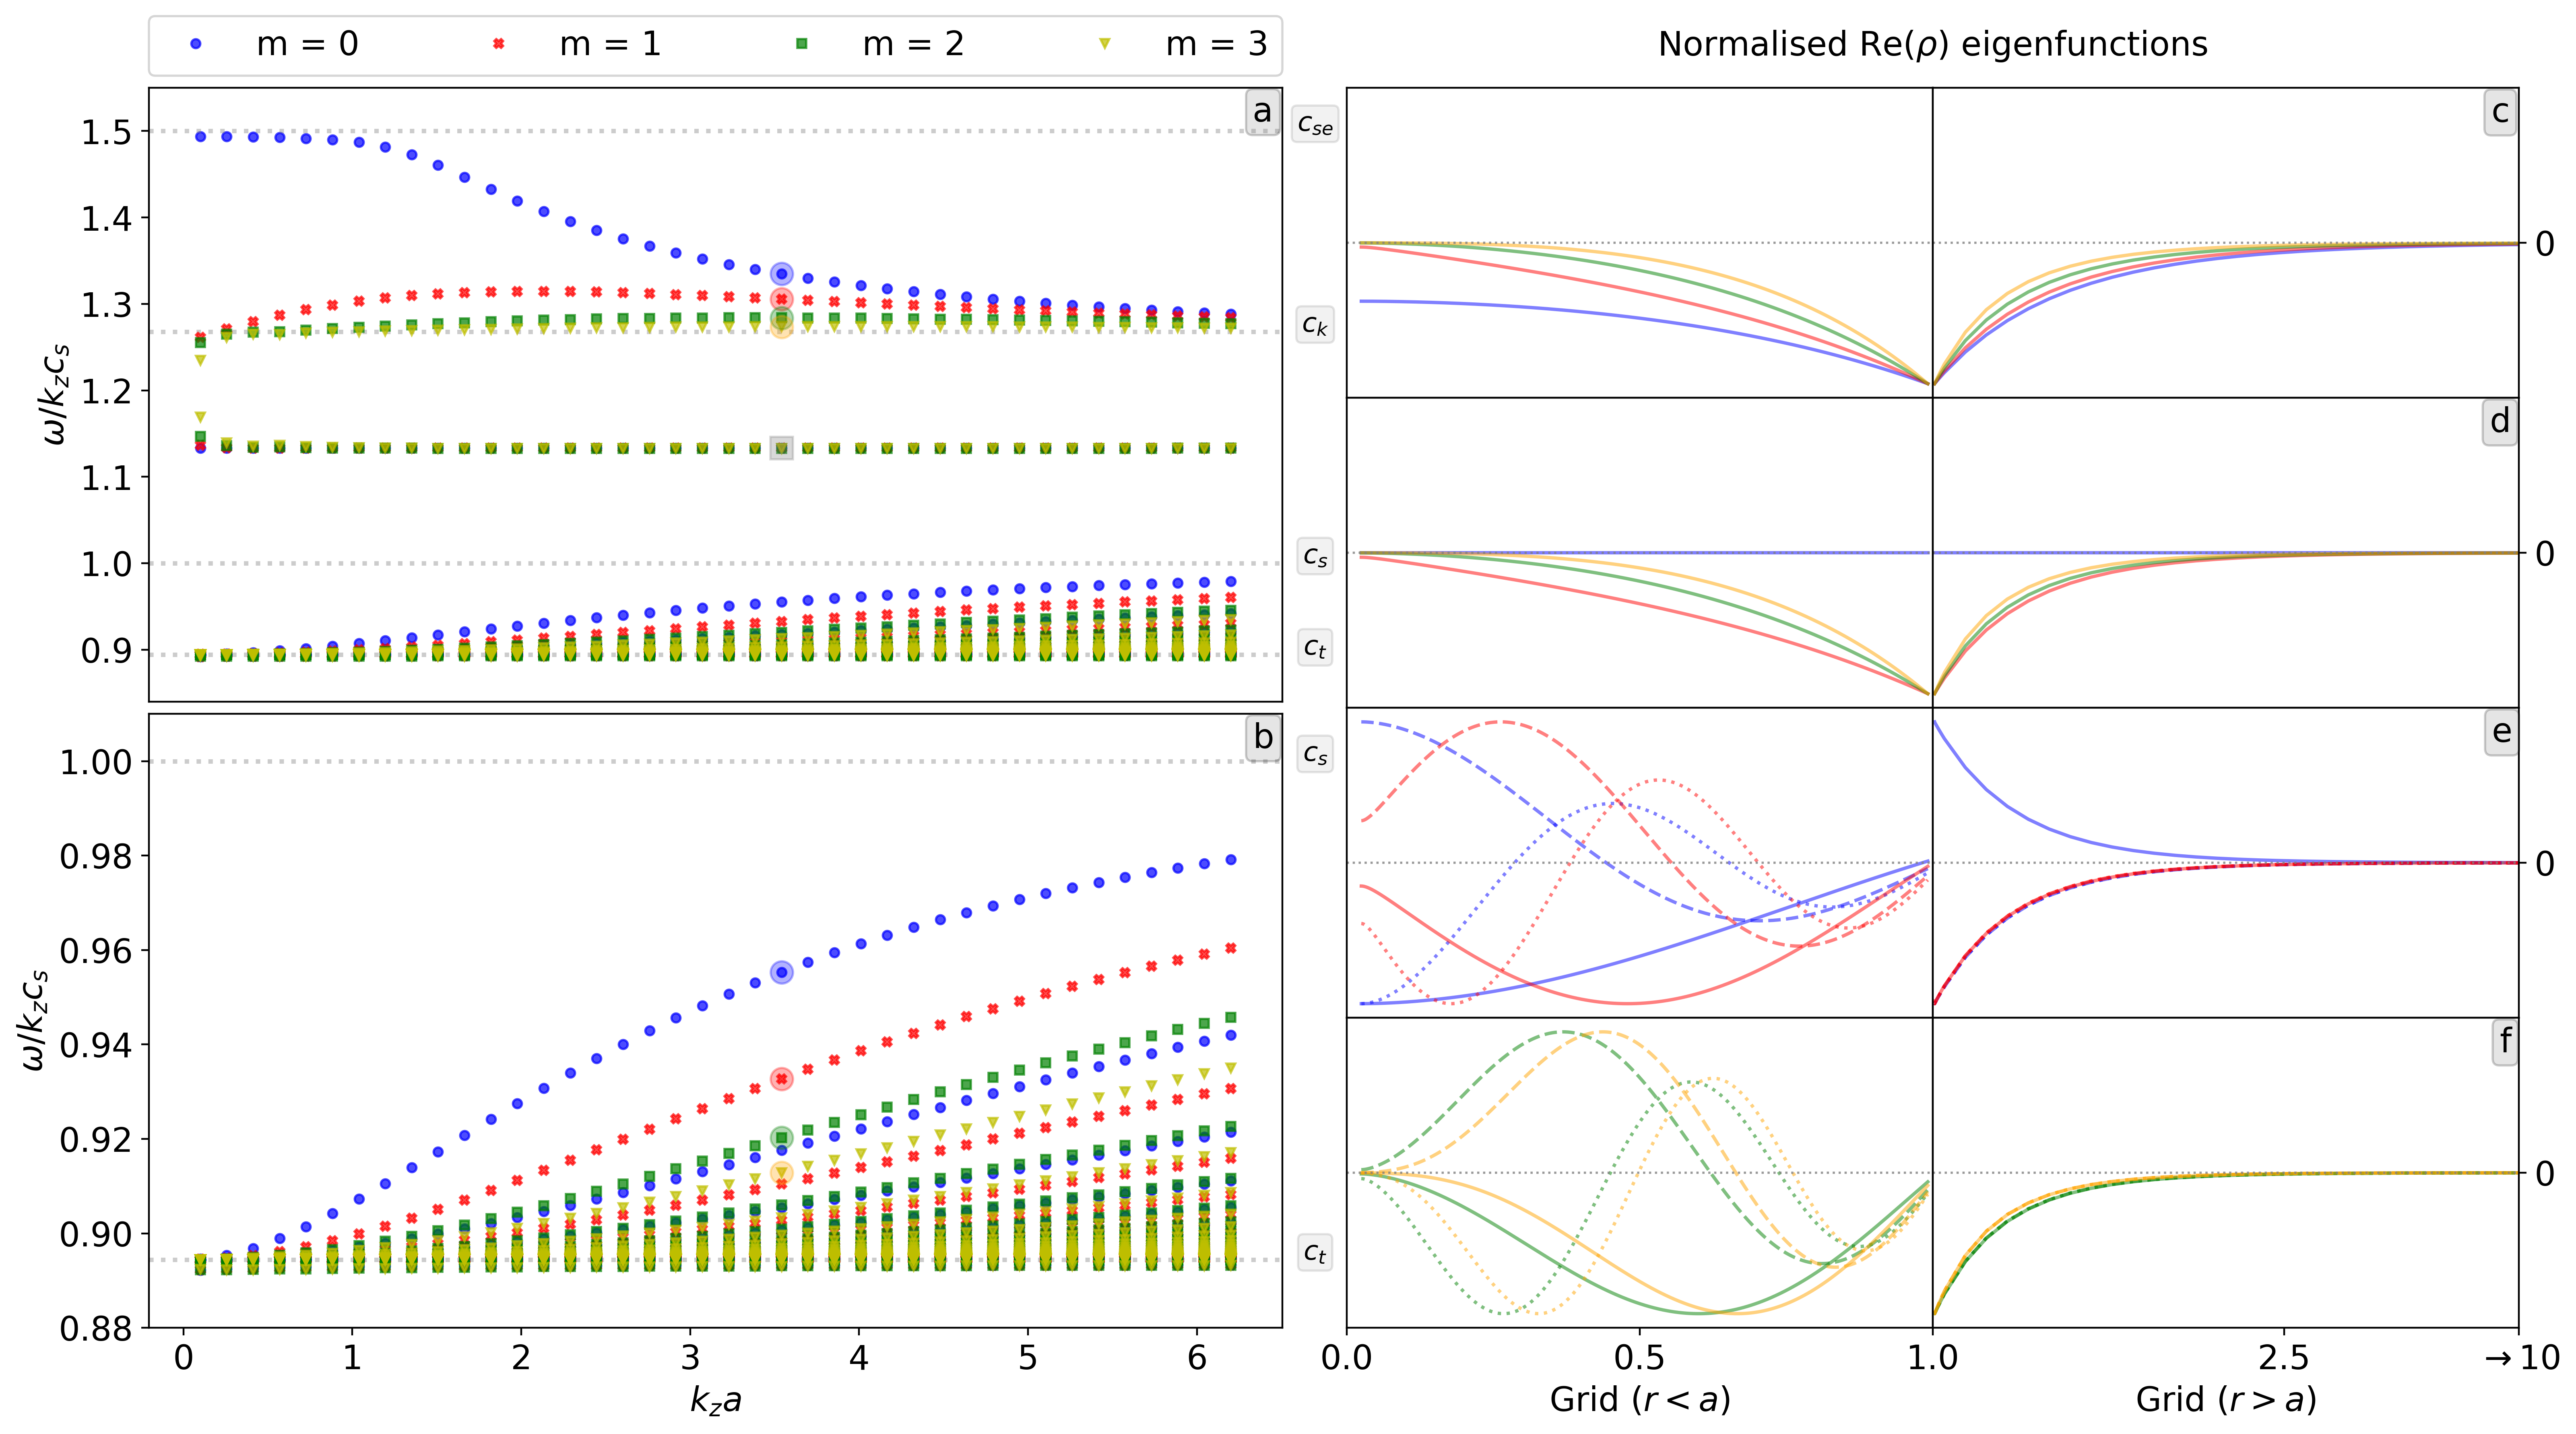
\includegraphics[width=\textwidth]{fluxtube_photospheric.png}
  \caption{
    Panel \textbf{a}: spectrum showing the dispersion relation for a flux tube under photospheric conditions. The dimensionless phase speed $\omega / k_z \soundspeed$ is displayed as a function of the dimensionless wavenumber $k_z a$ for four values of the azimuthal wavenumber $m = 0$ (blue dots), $m = 1$ (red crosses), $m = 2$ (green squares), and $m = 3$ (yellow triangles). Both sound speeds, the kink speed, and the tube speed are denoted using dashed grey horizontal lines, all normalised to $\soundspeed$. Panel \textbf{b}: zoom-in of Panel \textbf{a} between the tube speed $\tubespeed$ and internal sound speed $\soundspeed$. Panels \textbf{c} and \textbf{d}: eigenfunctions of the modes associated with circles (\textbf{c}) and squares (\textbf{d}) on the top-left Panel \textbf{a}. Panel \textbf{e}: first three eigenfunctions of the $m = 0$ and $m = 1$ body wave sequence on Panel \textbf{b}. Panel \textbf{f}: first three eigenfunctions of the $m = 2$ and $m = 3$ body wave sequence. For both panels \textbf{e} and \textbf{f}, the $n = 1$, $n = 2$, and $n = 3$ modes are shown in solid, dashed and dotted lines, respectively; only the first mode is annotated on the bottom-left Panel. Every eigenfunction in panels \textbf{c}--\textbf{f} is normalised to its maximum absolute value in that particular grid interval.
  }
  \label{fig: fluxtube_photospheric}
\end{figure}

All speeds indicated in the figure are normalised to the internal sound speed $\soundspeed$. Panel a clearly shows the fast surface waves, including the sausage $(m = 0)$, kink $(m = 1)$, and first two fluting modes ($m = 2$ and $m = 3$). The eigenfunctions in Panel c correspond to the modes annotated with a transparent circle in Panel a, with colours indicating the mode number $m$. The left and right sides of Panels c--f show the eigenfunctions for the inner and outer regions of the flux tube, respectively. All eigenfunctions are normalised to their maximum value, and all eigenvalues having a normalised phase speed larger than 1.5 are not shown. It should be noted that the first three runs, that is, the first three dots according to the $k_z a$ axis, were done using 1001 gridpoints. The reason for this is that when we divide the eigenvalues $\omega$ by $k_z$, small errors are increased selectively for small $k_z$, explaining why those modes seem slightly scattered and hence why he have to employ such high resolutions in order to minimise said error.

Panel b of Figure \ref{fig: fluxtube_photospheric} zooms in between the tube speed ($\tubespeed$) and internal sound speed ($\soundspeed$), showing a clear representation of the various body waves that accumulate to the tube speed at long wavelengths. Panel e shows the first three modes of the $m = 0$ and $m = 1$ sequences in solid, dashed, and dotted lines, respectively; that is, the first mode in the sequence (solid line) corresponds to the mode annotated in Panel b. The next two modes in that sequence are the next two blue dots moving vertically downwards (same $k_z a$ value), these are not annotated to avoid cluttering the figure. Analogously, Panel f shows the first three modes of the $m = 2$ and $m = 3$ sequences, with everything colour-coded according to the legend. As indicated before, all eigenfunctions in the outer region are exponentially varying. Panels a and b in Figure \ref{fig: fluxtube_photospheric} reproduce the analytical results in \citet[Figure 6.5]{book_roberts}.

One mode has not yet been discussed, and that is the horizontal line of modes between the internal sound speed and kink speed. The eigenfunctions are shown in Panel d and correspond to the annotated squares in the top-left Panel a. These modes are not present in the original work, and it is not a priori clear how to interpret them. These modes are degenerate, meaning that their position does not change when the mode number $m$ or wavenumber $k_z$ changes. The position of the outer wall also does not seem to have any influence on their value, and their eigenfunctions seem to indicate that these are surface waves. However, it is also quite possible that these modes are a numerical remnant of the discontinuous equilibrium profile, and are picked up by {\legolas} due to the sharp transition between the inner flux tube and the environment at $a = 1$.

\paragraph{(b) Coronal flux tube.} The second application of the magnetic flux tube is one under coronal conditions, that is, an equilibrium for which $c_\text{se} < \soundspeed < \alfvenspeed < c_\text{Ae}$. More specifically, we take
$c_\text{Ae} = 5\soundspeed$, $c_\text{se} = \soundspeed/2$, and $\alfvenspeed = 2\soundspeed$. Analogous to the previous case, the relations between the equilibrium values inside and outside of the flux tube follow from Equation \eqref{eq: flux_tube_pbalance}, where we again take $p_0$ and $\rho_0$ to be equal to one. This results in
$\rho_0 \approx 4.86~\rho_\text{e}$, $\tubespeed \approx 0.89~\soundspeed$, and
$\kinkspeed \approx 1.38~\alfvenspeed \approx 0.55~c_\text{Ae}$, and we use the same values as for the photospheric case for $k_z$ and the flux tube and outer wall boundaries. Similar to case (a), we perform 40 runs at 300 gridpoints each for four values of $k_2 = m$ (where again the first three runs have 1001 gridpoints) and plot the spectrum showing the dispersion relation in Figure \ref{fig: fluxtube_coronal}. Again, all speeds indicated in the figure are normalised to the sound speed $\soundspeed$. The top-left Panel a focuses on the fast body waves, the bottom-left Panel b on the slow body waves. Panel c shows the eigenfunctions corresponding to the four body waves indicated with circles in Panel a. Panel d depicts the eigenfunctions of the modes annotated with squares between the internal Alfv\'en ($\alfvenspeed$) and kink ($\kinkspeed$) speeds, representing the kink $m = 1$ and first two fluting ($m = 2$ and $m = 3$) modes.

\begin{figure}[t]
  \centering
  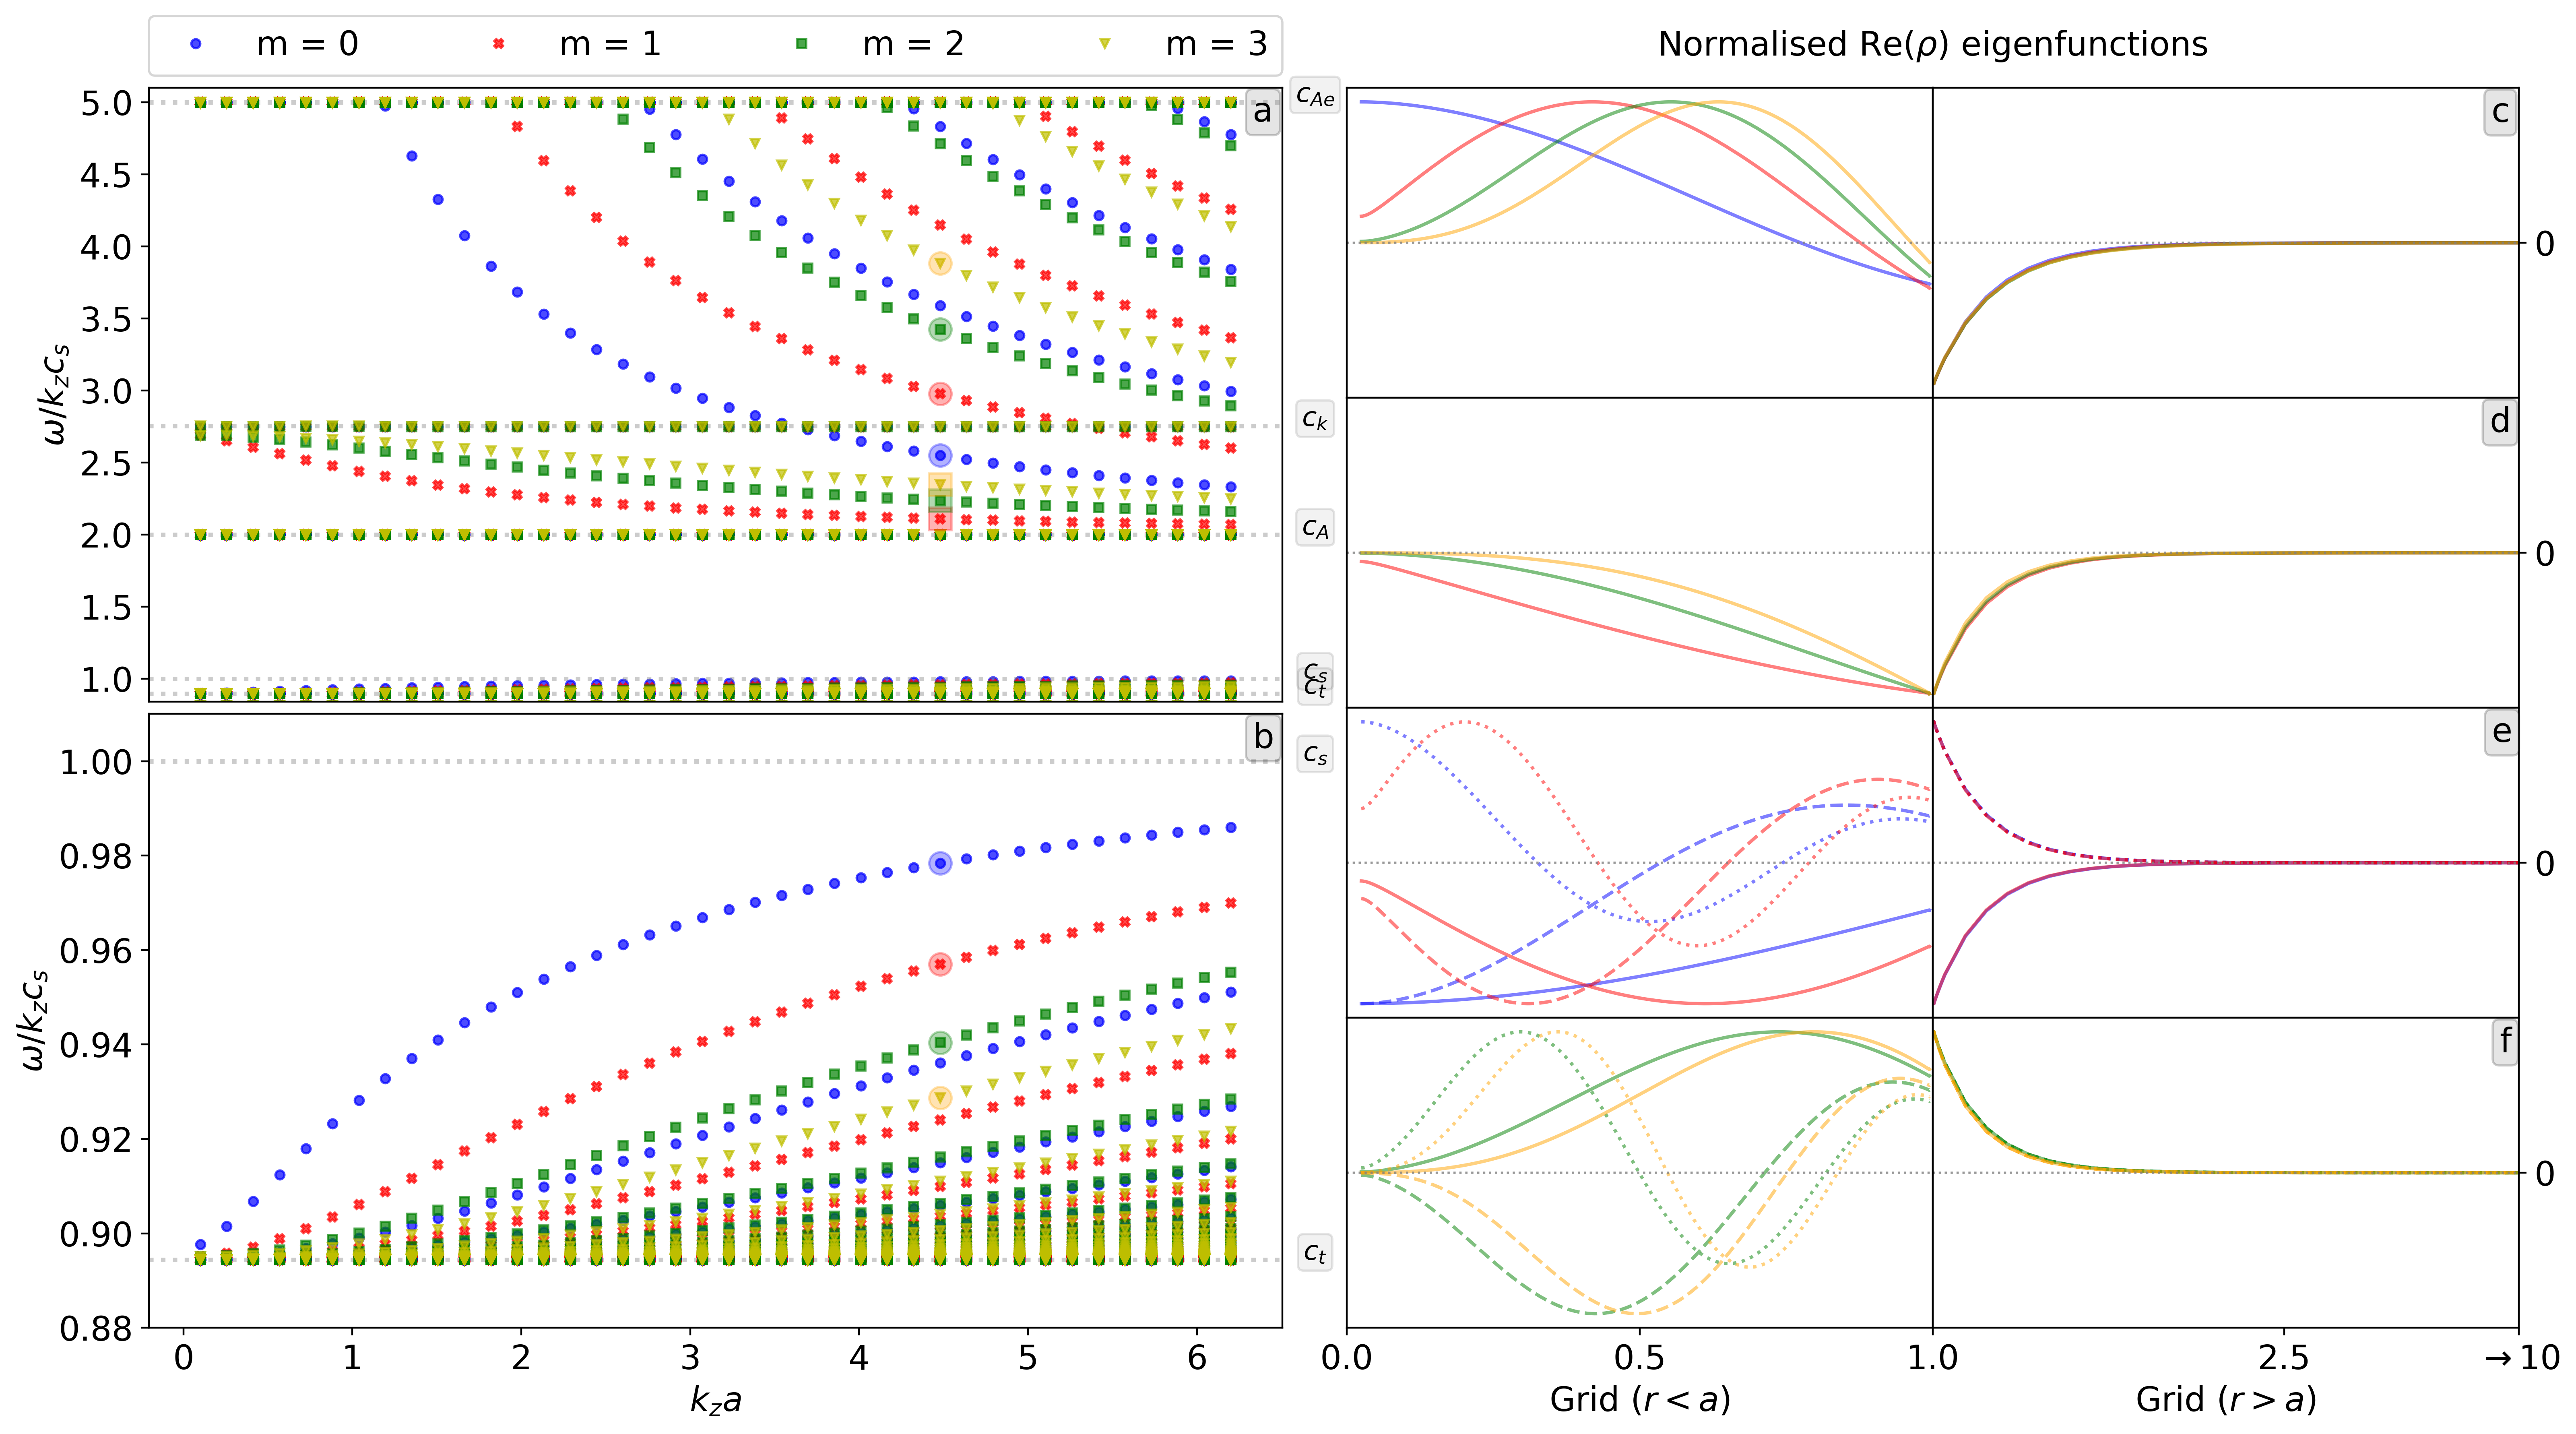
\includegraphics[width=\textwidth]{fluxtube_coronal.png}
  \caption{
    Panel \textbf{a}: spectrum showing the dispersion relation for a flux tube under coronal conditions. The dimensionless phase speed $\omega / k_z \soundspeed$ is displayed as a function of the dimensionless wavenumber $k_z a$ for four values of the azimuthal wavenumber $m = 0$ (blue dots), $m = 1$ (red crosses), and $m = 2$ (green squares), and $m = 3$ (yellow triangles). Both Alfv\'en speeds, together with the kink, tube, and sound speeds are denoted by grey horizontal lines and are all normalised to $\soundspeed$. Panel \textbf{b} zoom-in of Panel \textbf{a} between the tube speed $\tubespeed$ and internal sound speed $\soundspeed$, zooming in on the tube-speed-related body mode sequences. Panels \textbf{c} and \textbf{d}: eigenfunctions of the modes annotated with circles (\textbf{c}) and squares (\textbf{d}) on the top-left Panel \textbf{a}. Panel \textbf{e}: first three eigenfunctions of the $m = 0$ and $m = 1$ body wave sequence in the bottom-left Panel \textbf{b}. Panel \textbf{f}: first three eigenfunctions of the $m = 2$ and $m = 3$ body wave sequence. For both Panels \textbf{e} and \textbf{f} the $n = 1$, $n = 2$ and $n = 3$ modes are shown in solid, dashed and dotted lines, respectively, only the first mode is annotated on Panel \textbf{b}. Every eigenfunction in Panels \textbf{c}--\textbf{f} is normalised to its maximum absolute value in that particular grid interval.
  }
  \label{fig: fluxtube_coronal}
\end{figure}

Similar to Figure \ref{fig: fluxtube_photospheric}, Panels e and f represent the first three body modes in the $m = 0$ and $m = 1$ sequences (Panel e), of which the first mode is indicated in Panel b. Panel f shows the first three modes of the $m = 2$ and $m = 3$ sequences, with the first, second, and third modes indicated with a solid, dashed and dotted line, respectively. The colours of Panels c--f are consistent with the legend. Figure \ref{fig: fluxtube_coronal} reproduces the analytical results in \citet[Figure 6.7]{book_roberts}, which are based on the analytic dispersion relation containing Bessel functions.

\subsection{Tokamak current profile}
Next we discuss an example initially given in \citet{kerner1985}, which shows the ideal MHD spectrum in the presence of an unstable $m = -2$ interchange mode in a cylindrical geometry. We start from a so-called tokamak current profile, in which an axial current density of the form $\boldsymbol{j}_0 = \left(0, 0, j_0(1 - r^2)^\nu\right)$ is assumed, with $j_0$ a given constant. This yields a twisted magnetic field profile in which the longitudinal component $B_{0z}$ is uniform and equals one, while the poloidal component $B_{0\theta}$ is given by
\begin{equation} \label{eq: tokamak_btheta}
  B_{0\theta} = \frac{j_0}{2r\left(\nu + 1\right)}\left[1 - \left(1 - r^2\right)^{\nu + 1}\right],
\end{equation}
for a given value of $\nu$. For the equilibrium considered here, we take $\nu = 0$, making the current profile constant over the flux tube. This means that $B_{0\theta}$ has a linear profile in $r$ such that the magnetic field lines have a constant pitch and the current is distributed equally in the plasma. An expression for the pressure (and hence temperature) can be found by integrating the force-balance Equation \eqref{eq: force_equilibrium} and assuming that, for example, the pressure vanishes at the outer boundary, resulting in a parabolic pressure profile. Hence, for a cylindrical geometry in which $r \in [0, 1]$, this yields the following equilibrium configuration:
\begin{equation}
  \begin{gathered}
    \rho_0 = 1,
    \qquad
    p_0 = \frac{1}{4}j_0^2\left(1 - r^2\right),
    \qquad
    B_{02} = \frac{1}{2}j_0 r,
    \qquad
    B_{03} = 1,
  \end{gathered}
\end{equation}
where we assumed a uniform density. We introduce an additional parameter $q$, called the \emph{safety factor}, given by
\begin{equation}
  q(r) = \frac{rk_z B_{0z}}{B_{0\theta}} = \frac{2k_z}{j_0}.
\end{equation}

We performed 39 runs, varying the $q$ factor between 1.9 and 2.1 in order to probe the regime containing the unstable $m = -2$ interchange mode, which is associated with the vanishing of the factor $m + kq$, that is, the $\bk \cdot \bb$ product. This implicitly constrains the value for $j_0$, and we assigned $k_2 = m = -2$ and $k_3 = k = 0.2$ for all runs. It should be noted that this particular equilibrium configuration requires a relatively high resolution near $q = 2$ to correctly resolve the unstable modes; here we used 501 gridpoints for all runs. The complete spectrum is shown in Figure \ref{fig: tokamak_current}, where the squared eigenvalues are plotted as a function of the safety factor. The three main branches, that is, fast, Alfv\'en and slow, are denoted on the right side of the figure, as well as the region where the modes become unstable $(\omega^2 < 0)$. We see that in the region near the $m = -2$ interchange instabilities, the slow and Alfv\'en modes collapse to zero, which is due to the vanishing of the combination $\Fplus$ (see Equation \eqref{eq: F_G_operators} in Chapter \ref{ch: Legolas}) in the ideal MHD equations \citep{book_MHD}. The slow and Alfv\'en continua are annotated in the figure in red and cyan, respectively. The Alfv\'en continuum is collapsed to a single point for this equilibrium configuration, while the slow continuum covers a range in frequency. Note in particular how the full spectrum ranges over many orders of magnitude in the $\omega^2$ view shown here: an intrinsic property (and challenge!) posed by MHD spectral theory.

\begin{figure}[t]
  \centering
  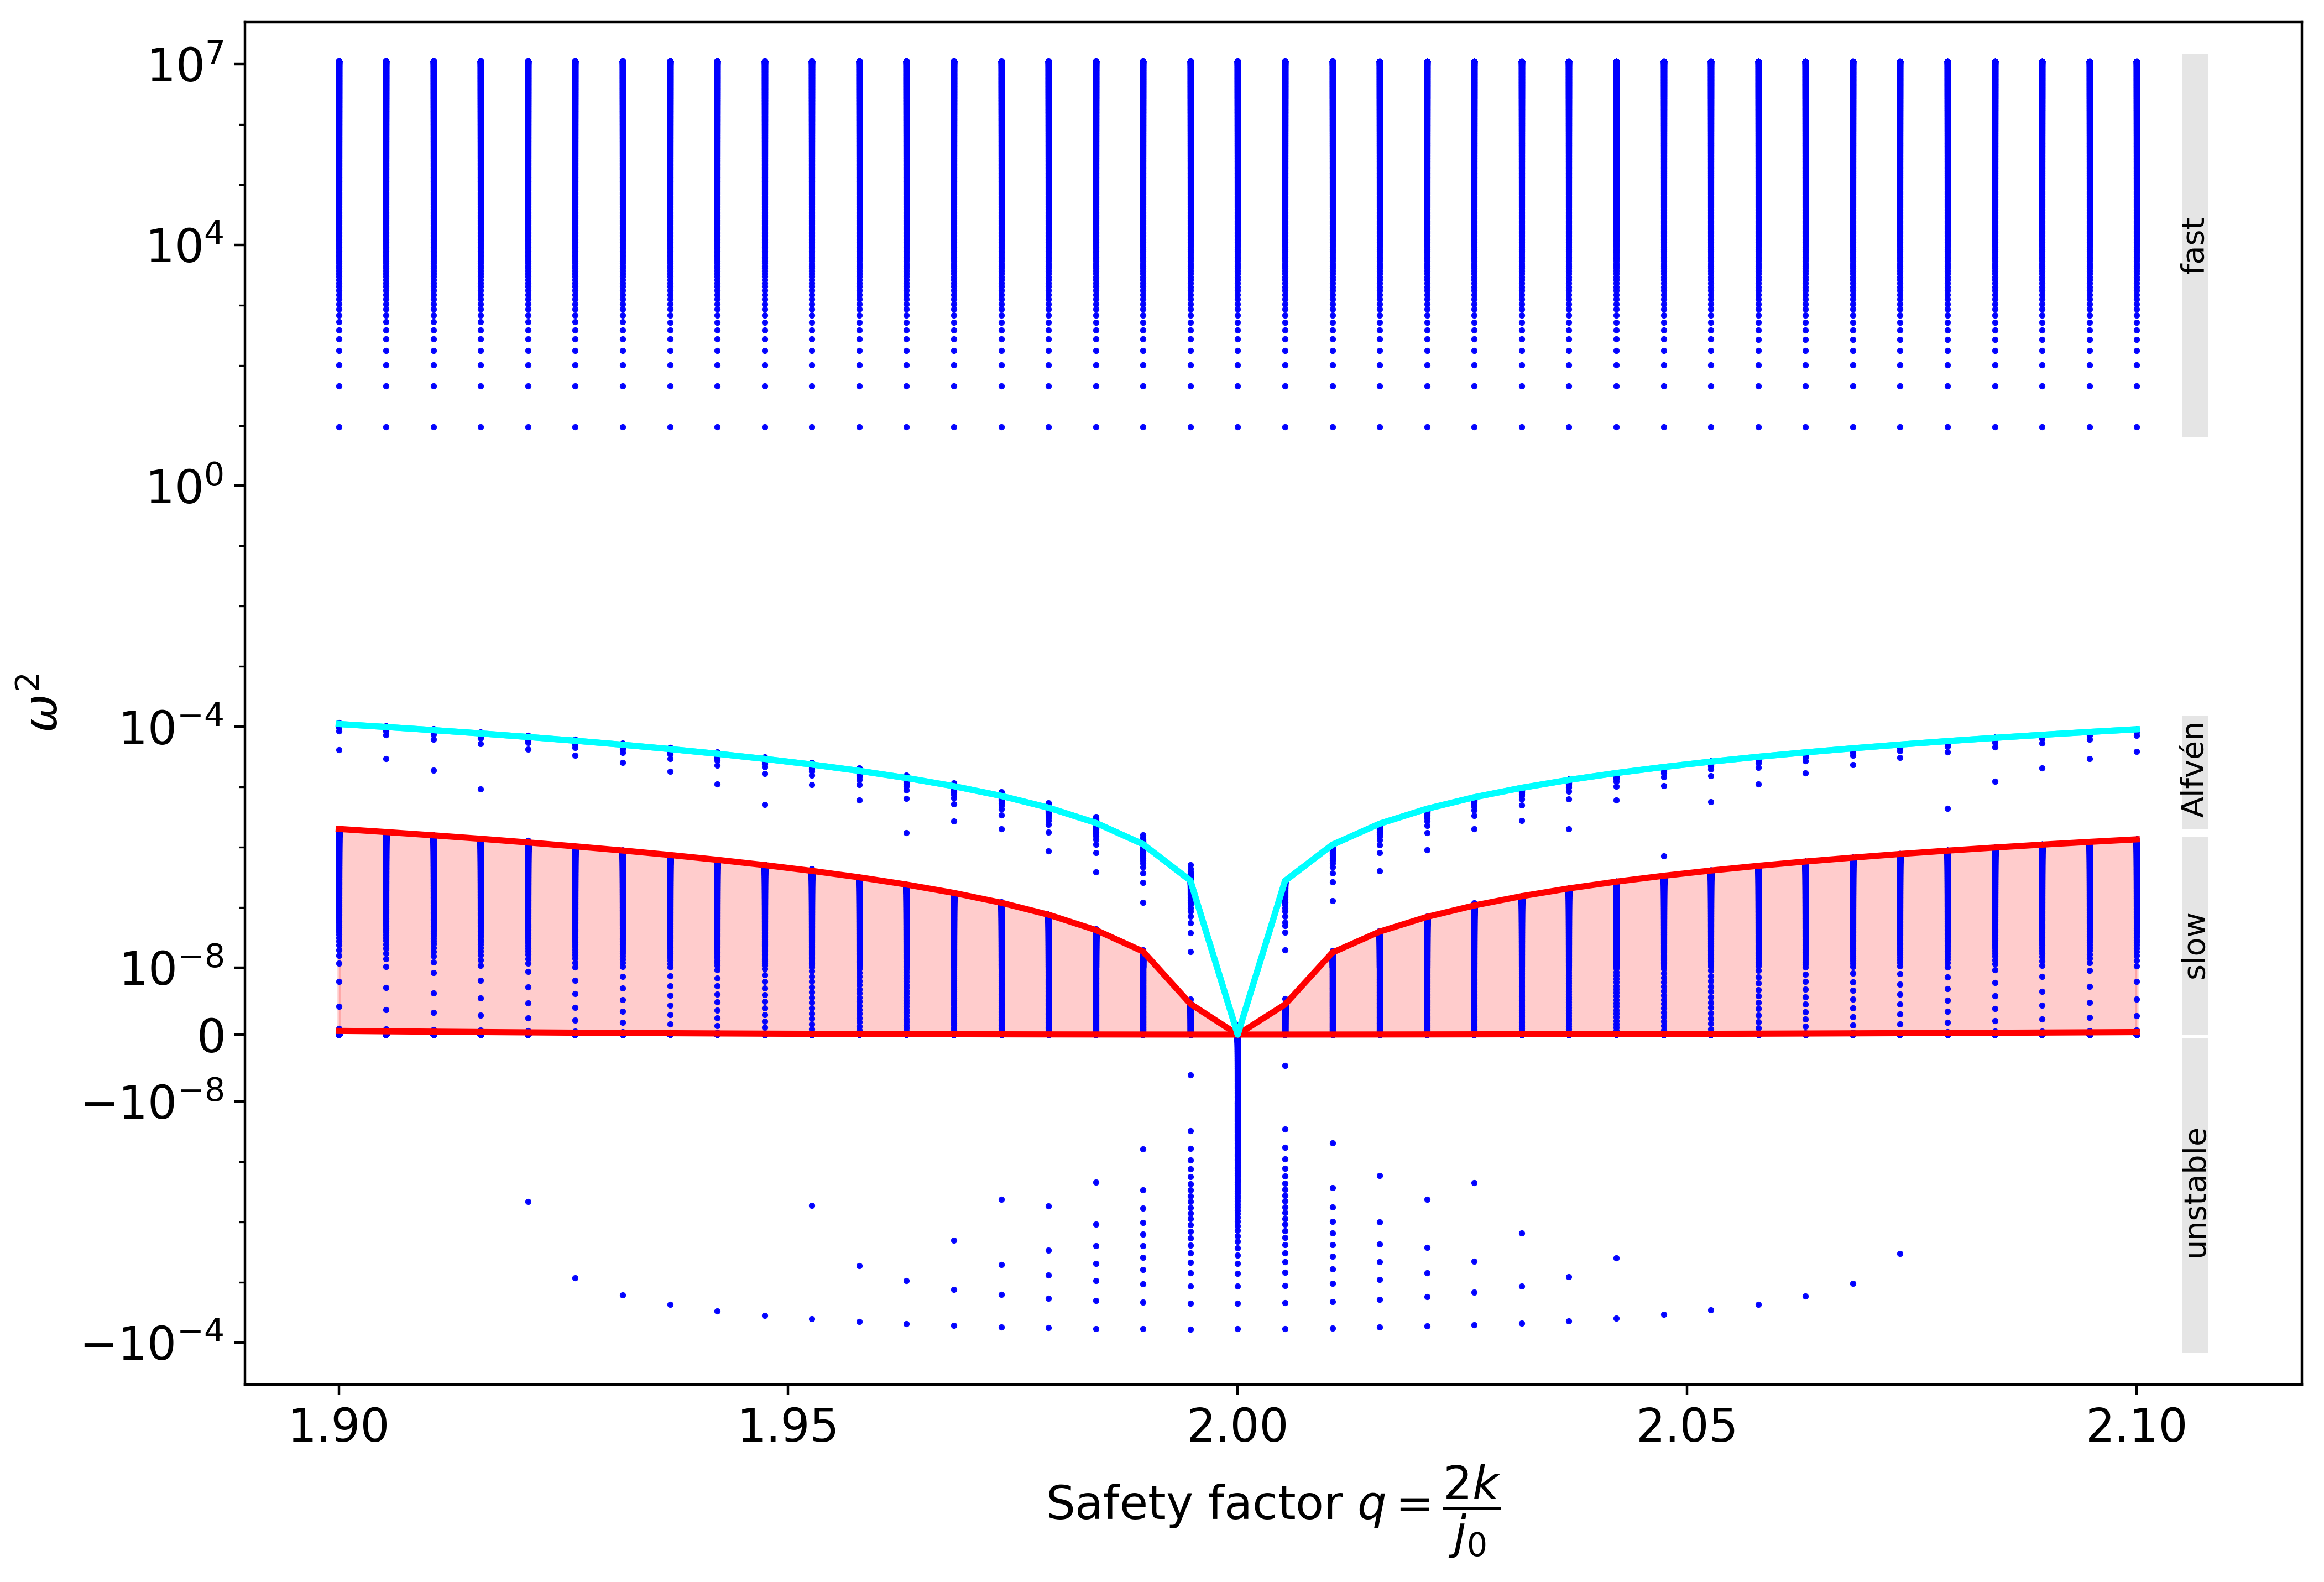
\includegraphics[width=\textwidth]{kerner_tokamak.png}
  \caption{
    Complete MHD spectrum for a tokamak current profile in the presence of the $m = -2$ interchange mode. The squared eigenvalues are plotted against the safety factor $q$, instabilities correspond to $\omega^2 < 0$. The various branches are indicated on the right side of the figure.
  }
  \label{fig: tokamak_current}
\end{figure}

\subsection{KH and CD instabilities}
As a first test for the inclusion of flow into the equations, we look at the interaction between the KHIs and current-driven (\gls{CD}) instabilities in a magnetised astrophysical jet, following \citet{baty2002}. This model uses a cylindrical jet with a supersonic background flow aligned with the axis and sheared in the radial direction. The equilibrium configuration is taken such that Kelvin-Helmholtz surface modes can develop and is generally given by
\begin{equation} \label{eq: kh_cd_equilibrium}
  \begin{gathered}
    \rho_0 = 1,
    \qquad
    v_{02} = 0,
    \qquad
    v_{03} = \frac{1}{2}\mathcal{V}\tanh\left(\frac{r_j - r}{a}\right), \\
    B_{02} = B_{0\theta} \frac{r r_c}{r_c^2 + r^2},
    \qquad
    B_{03} = B_{0z}, \\
    T_0 = \frac{p_0}{\rho_0} - \frac{B_{0\theta}^2}{2\rho_0}\left(1 - \frac{r_c^4}{\left(r_c^2 + r^2\right)^2}\right).
  \end{gathered}
\end{equation}
Here, $r_j$ denotes the jet radius and $r_c$ quantifies the radial variation, taken to be $r_j = 1$ and $r_c = 0.5$, with $r \in [0, 2]$. The parameter $\mathcal{V}$ represents the amplitude of the velocity, given by $\mathcal{V} = 1.63$, while the chosen velocity profile ensures that the shear layer is situated at the jet radius with a radial width given by $a = 0.1r_j$. Both the density $\rho_0$ and the pressure on-axis $p_0$ are chosen to be equal to unity. The parameters $B_{0\theta}$ and $B_{0z}$ control the amplitude and twist of the magnetic field, as explained in \citet{baty2002}. The original work discusses three different magnetic field configurations, we choose the profile with
\begin{equation}
  B_{0\theta} = 0.4\left(\frac{r_c^2 + r_j^2}{r_j r_c}\right),
  \qquad
  B_{0z} = 0.25,
\end{equation}
such that $B_{02} = 0.4$ at the jet radius. Furthermore, the azimuthal and longitudinal wavenumbers are taken to be $k_2 = m = -1$ and $k_3 = k = \pi$.

The entire spectrum is calculated using 501 gridpoints and shown in Figure \ref{fig: kh_cd}. Panel a depicts the full slow and Alfv\'en spectra with the KH and first three CD unstable modes ($\omega_\text{I} > 0$) denoted on the figure itself. The real and imaginary parts of the $\rho$, $r v_r$, and $v_z$ eigenfunctions for each of these modes are shown on the subsequent panels. Those for the KH mode (Panels c--d) are localised around the jet radius $r = 1$, which is also the point where the Alfv\'enic Mach number drops to zero (Panel b). The quantity $V_0$ in the Figure legend represents the velocity magnitude, here given by $V_0 = \sqrt{v_{02}^2 + v_{03}^2}$. Panels e through j depict the eigenfunctions of the first three CD modes, with the first, second, and third shown in the first, second, and third rows of the bottom panels, respectively. The left column shows the real part, the right column the imaginary part of the eigenfunction. The CD modes have an increasing number of nodes on $r \in [0, 1]$, which is most clearly visible by looking at the
$r v_r$ eigenfunction (green): no nodes for the first CD mode (Panels e--f), one node for the second CD mode (Panels g--h), and two nodes for the third CD mode (Panels i--j).

\begin{figure}[t]
  \centering
  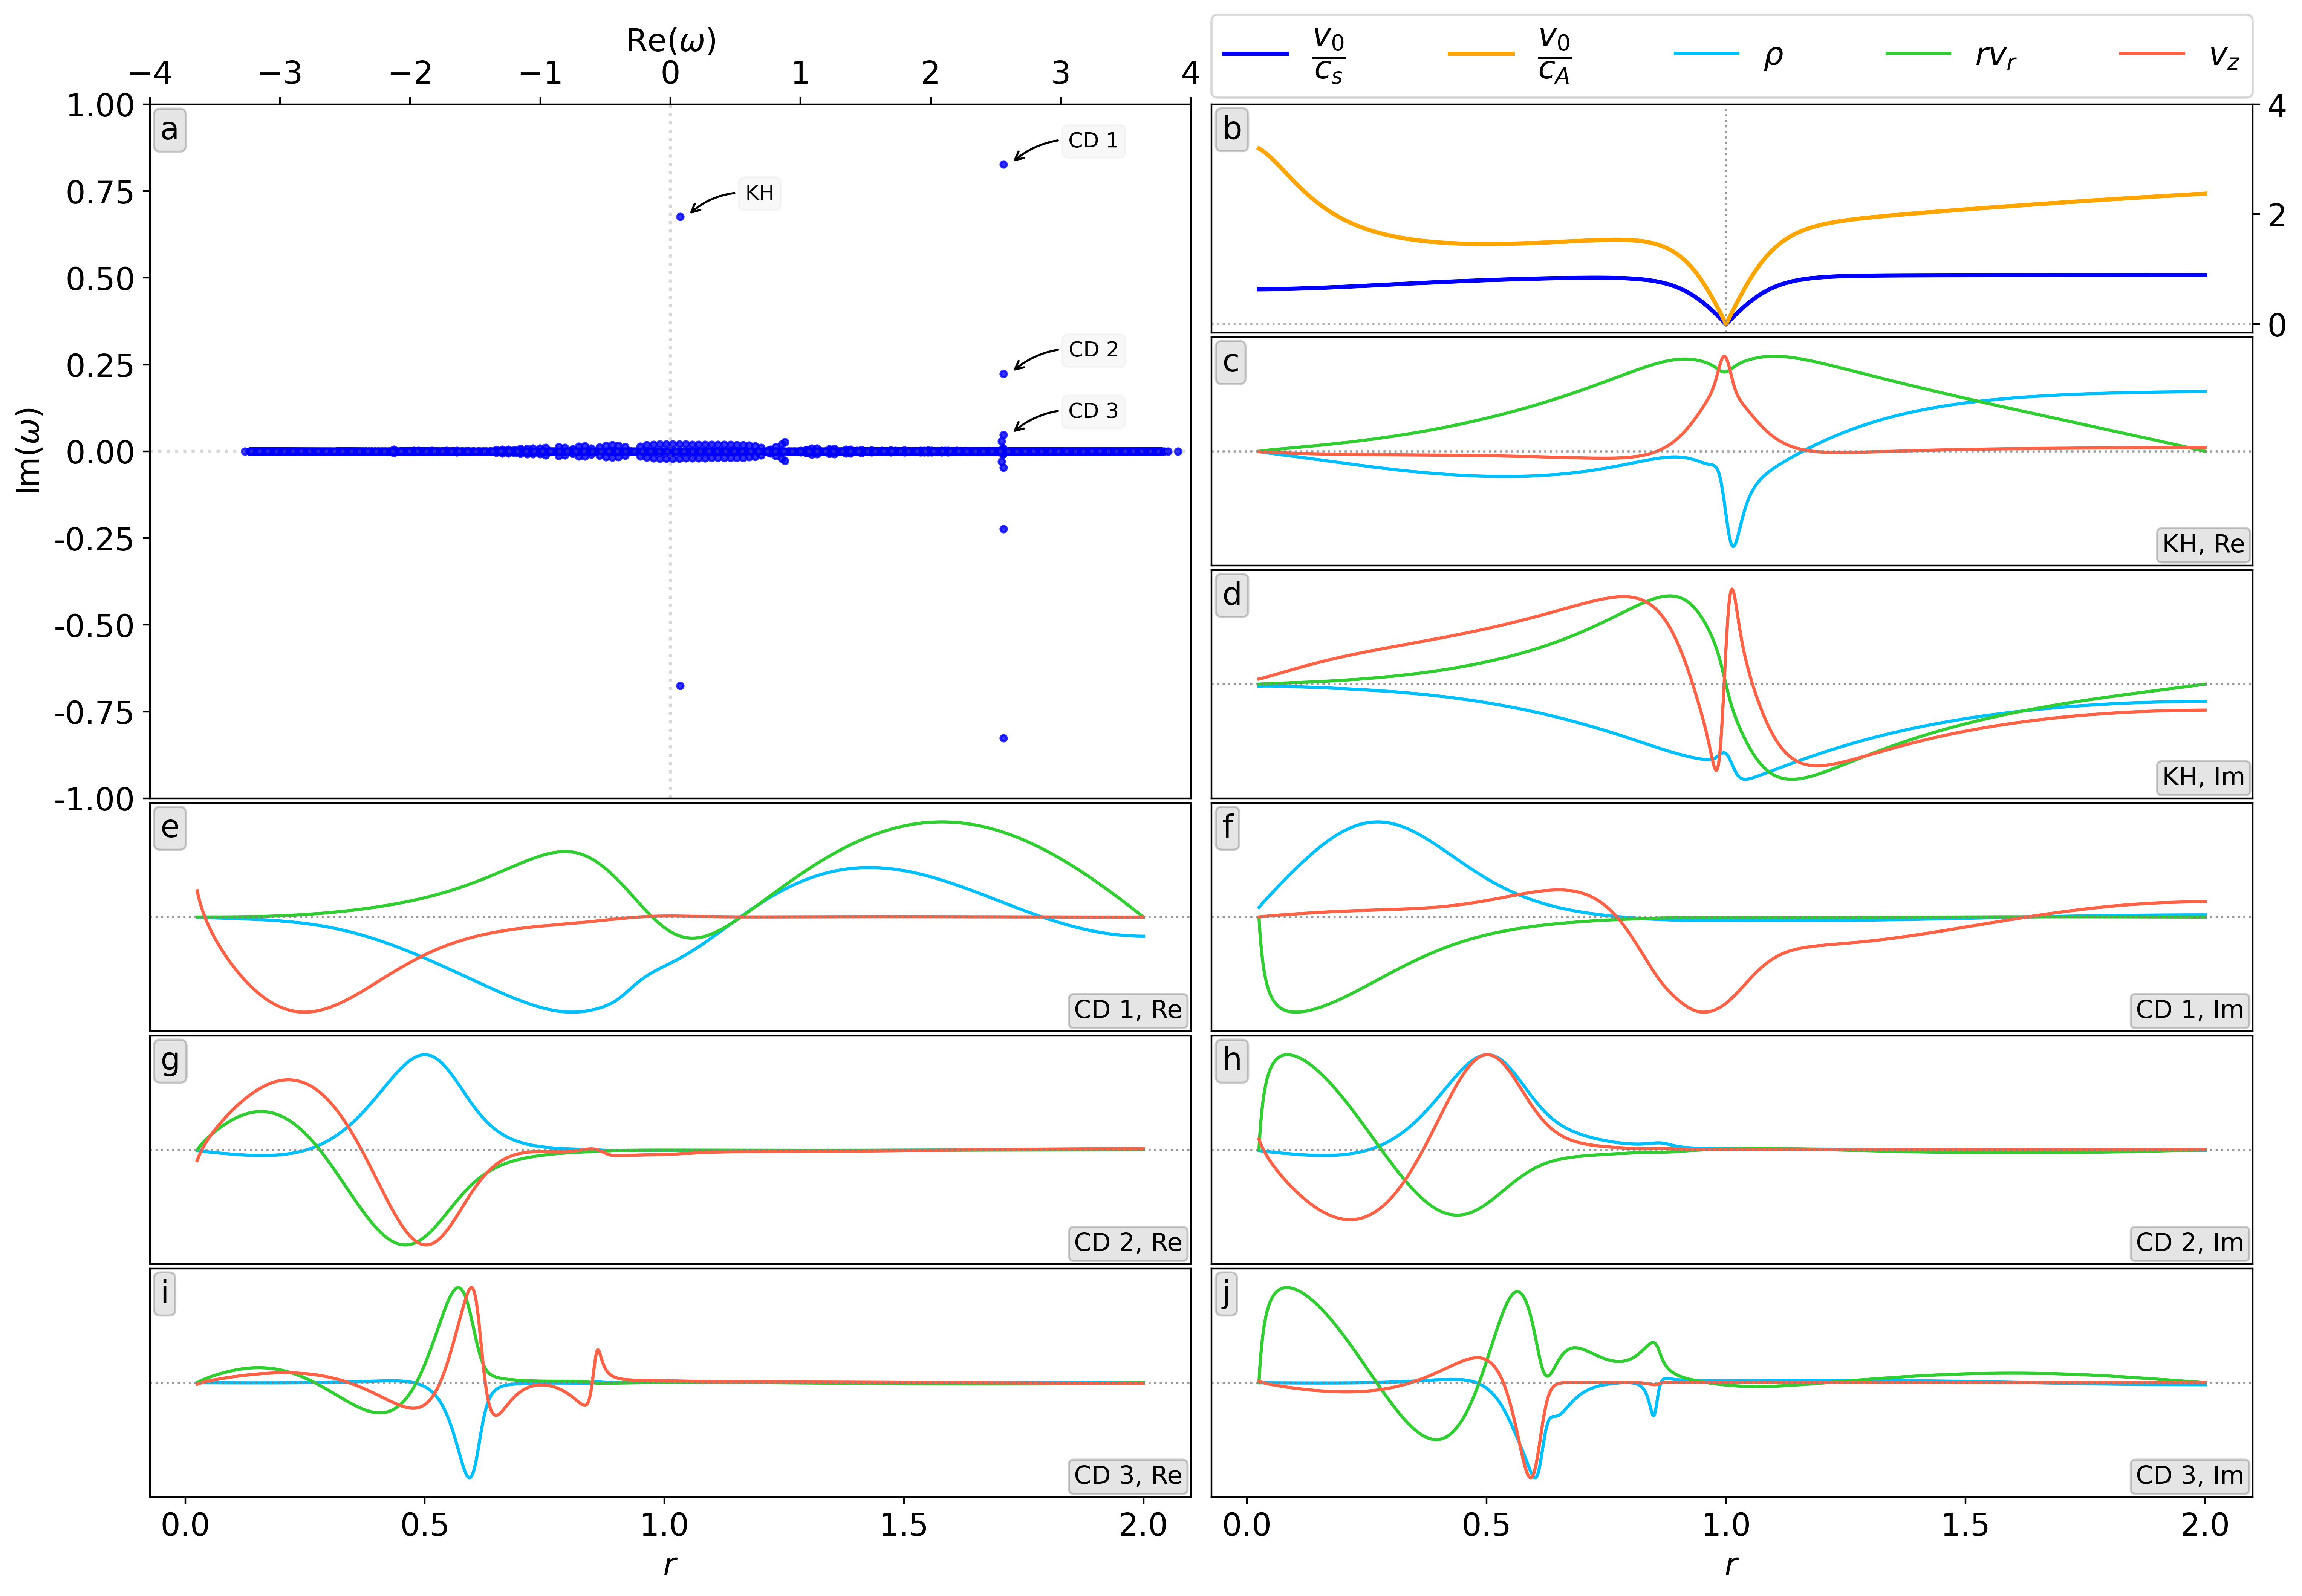
\includegraphics[width=\textwidth]{kh_cd.png}
  \caption{
    Panel \textbf{a}: MHD spectrum for the equilibrium configuration given in \eqref{eq: kh_cd_equilibrium}. The KH and CD instabilities are indicated on the panel. Panel \textbf{b}: sonic and Alfv\'enic Mach numbers; the other panels show the real and imaginary parts of the $\rho$ (blue), $r v_r$ (green) and $v_z$ (red) eigenfunctions, for the KH mode (Panels \textbf{c} and \textbf{d}), first CD mode (Panels \textbf{e}--\textbf{f}), second CD mode (Panels \textbf{g}--\textbf{h}), and third CD mode (Panels \textbf{i}--\textbf{j}).
  }
  \label{fig: kh_cd}
\end{figure}

Note that here, we are still in adiabatic conditions such that the up-down symmetry (relating to time reversal) is still present in the eigenfrequency plane, but the introduction of equilibrium flow caused left-right symmetry breaking between the forwards and backwards propagating modes. As pointed out in \citet{goedbloed2018_web1}, the study of MHD spectra of stationary (i.e. with flow) equilibria is still governed by two self-adjoint operators, but as seen in Figure \ref{fig: kh_cd}, modes can enter the complex plane at various locations (identified by the spectral web; \citet{goedbloed2018_web2}). The correspondence with the original figure in \citet{baty2002} is one-to-one for the KH and CD modes, but here we have a lot more detail near the axes due to the (much) higher resolution employed. This resolution aspect will be further discussed in Section \ref{sec: convergence}.

\subsection{Suydam cluster modes}

\section{Resistive, Cartesian cases}
\subsection{Resistive homogeneous plasmas}
\subsection{Quasi-modes in resistive MHD}
\subsection{Resistive tearing modes}
\subsection{Tearing modes with varying resistivity}

\section{Nonadiabatic, cylindrical cases}
\subsection{Nonadiabatic discrete Alfv\'en waves}
\subsection{Magnetothermal instabilities}

\section{Convergence} \label{sec: convergence}

\section{The Legolas testing framework}

\section{Discussion}





\cleardoublepage
